% !TEX program = xelatex
\documentclass[a4paper, UTF8, fontset=adobe]{ctexart}

\usepackage[left=2.50cm, right=2.50cm, top=2.50cm, bottom=2.50cm, headheight=14pt]{geometry}

\usepackage[unicode=true,colorlinks,urlcolor=blue,linkcolor=blue,bookmarksnumbered=true]{hyperref}
\usepackage{latexsym,amssymb,amsmath,amsbsy,amsopn,amstext,amsthm,amsxtra,color,bm,calc,ifpdf}
\usepackage{graphicx}
\usepackage{enumerate}
\usepackage{fancyhdr}
\usepackage{multirow}
\usepackage{makeidx}
\usepackage{fontspec}
\usepackage{pythonhighlight}
\usepackage{caption} % 用于自定义标题
\usepackage{titlesec} % 自定义标题格式
\usepackage{fmtcount} % 引入fmtcount宏包
\usepackage{tocloft} % 加载tocloft宏包
\usepackage{mathtools} % 引入mathtools包
\usepackage{bm}  % 导入 bm 宏包用于粗体希腊字母


\pagestyle{fancy}
\fancyhead[L]{}
\fancyhead[C]{Formula Derivation of R-VIO}
\fancyhead[R]{}

% 自定义section命令的格式
\titleformat{\section} % 命令
{\normalfont\Large\bfseries} % 格式化
{\thesection} % 编号
{0.5em} % 编号和标题文本之间的距离
{\raggedright} % 左对齐

% 设置目录中编号与标题之间的距离
\setlength{\cftsecnumwidth}{0.5em} % 设置节编号的宽度

\begin{document}
	
\tableofcontents % 生成目录

\thispagestyle{empty}

\newpage
\pagenumbering{arabic}

\section{Estimator design}
与标准的world-centric VINS不同,robocentric VINS使用local frame $\{R\}$用于导航,观测特征也在local frame下表示。
Frame $\{I\}$表示IMU坐标系,其与机器人坐标系$\{R\}$重合,因此global frame $\{G\}$(与初始的local frame $\{R_0\}$
重合)可以将相对于$\{R\}$的特征转换为静止特征。在导航过程中,$\{R\}$不断地从从一个IMU frame变换到另一个IMU frame。
坐标系示意图如Figure 1.1。原先的VINS滤波器公式都是相对于fixed global frame的,相对于local frame的VINS滤波器公式
需要重新组织。

\begin{figure}[ht]
\centering
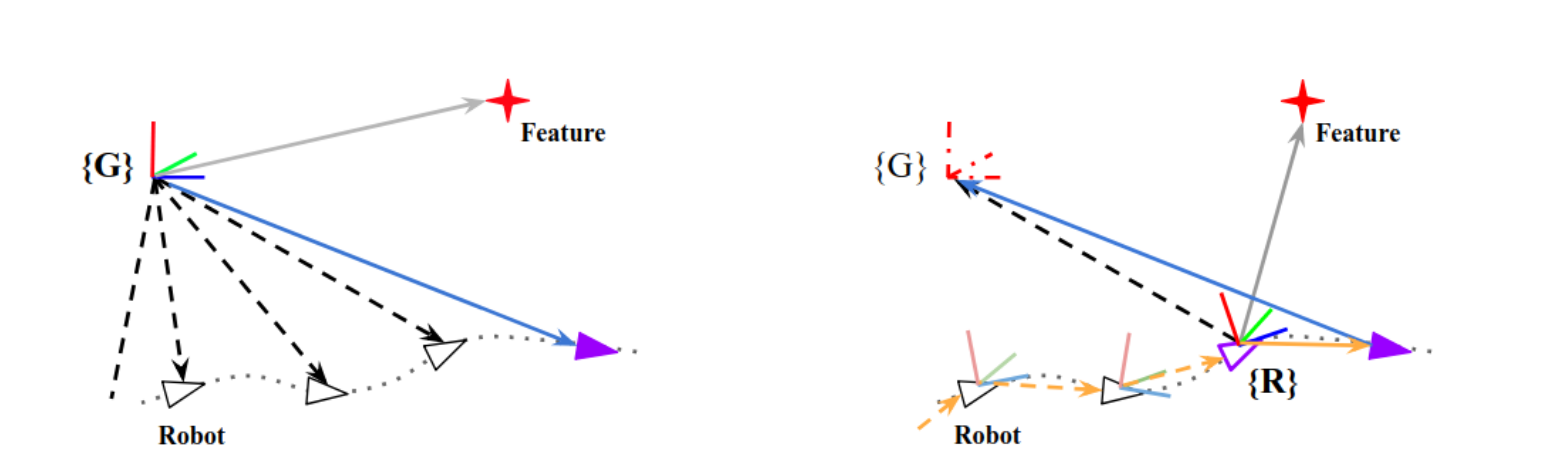
\includegraphics[width=0.65\textwidth]{figures/robocentric formulation illustration.png}
\captionsetup{labelformat=empty}
\caption{Figure 1.1: World-centric vs. robocentric formulation}
\end{figure}

\subsection{State vector}
R-VIO的state vector包含两个部分,(i)global frame,其维护了全局的运动信息;(ii)IMU state,其维护了从local frame of
reference到当前IMU frame的运动信息。在这个文档中,$k,k+1,...$表示图像的time-steps,$\tau - 1,\tau,...$表示两个连续
图像帧之间的IMU的time-steps,下标$\ell | i$表示在所有time-step $i$的测量都被处理之后,一个量在time-step $\ell$的估计。
$\hat{x}$表示随机变量$x$的估计,$\tilde{x}=x-\hat{x}$是这个估计的加性误差。$\mathbf{I}_n$和$\bm{0}_n$是
$n\times n$的单位阵和零矩阵。最后左边的上标表示该向量是在哪个frame表达。

% \[ 和 \] 是用来开始和结束一个展示数学环境的
特别的,在时刻$t_{\tau}\in \left[t_k,t_{k+1}\right]$,local frame $\{R_k\}$下,state给出如下:

\begin{equation}
\begin{aligned}
\numberwithin{equation}{section} % 公式编号将跟随章节编号
& \prescript{R_k}{}{\mathbf{x}_{\tau}} = \begin{bmatrix} \prescript{R_k}{}{\mathbf{x}^{\top}_G} & 
  \prescript{R_k}{}{\mathbf{x}^{\top}_{I_{\tau}}} \end{bmatrix}^{\top}, \\
& \prescript{R_k}{}{\mathbf{x}_G} = \begin{bmatrix} \prescript{k}{G}{\bar{q}^{\top}} & 
  \prescript{R_k}{}{\mathbf{p}^{\top}_G} & \prescript{R_k}{}{\mathbf{g}^{\top}} \end{bmatrix}^{\top}, \\
& \prescript{R_k}{}{\mathbf{x}_{I_{\tau}}} = \begin{bmatrix} \prescript{\tau}{k}{\bar{q}^{\top}} & 
  \prescript{R_k}{}{\mathbf{p}^{\top}_{I_{\tau}}} & \mathbf{v}^{\top}_{I_{\tau}} &
  \mathbf{b}_{g_{\tau}}^{\top} & \mathbf{b}_{a_{\tau}}^{\top} \end{bmatrix}^{\top} 
\end{aligned}
\end{equation}

\noindent 这里$\prescript{k}{G}{\bar{q}}$是一个表示frame $\{G\}$在frame $\{R_k\}$下姿态的单位四元数,
$\prescript{R_k}{}{\mathbf{p}_G}$是frame $\{G\}$在frame $\{R_k\}$下的位置;$\prescript{\tau}{k}{\bar{q}}$和 
$\prescript{R_k}{}{\mathbf{p}_{I_{\tau}}}$是从frame $\{R_k\}$到frame $\{I_{\tau}\}\}$的相对的旋转和平移;
$\mathbf{v}_{I_{\tau}}$是在frame $\{I_{\tau}\}\}$表达的local velocity,$\mathbf{b}_{g_\tau}, \mathbf{b}_{a_\tau}$
分别是陀螺仪和加速度计的偏置。需要注意的是,local gravity $\prescript{R_k}{}{\mathbf{g}}$也是系统状态的一部分,其
是一个大小固定(e.g. 9.81)的$3\times1$的向量。

\noindent 对应的error state由下式给出:

\begin{equation}
\begin{aligned}
\numberwithin{equation}{section} % 公式编号将跟随章节编号
& \prescript{R_k}{}{\tilde{\mathbf{x}}_{\tau}} = \begin{bmatrix} \prescript{R_k}{}{\tilde{\mathbf{x}}^{\top}_G} & 
\prescript{R_k}{}{\tilde{\mathbf{x}}^{\top}_{I_{\tau}}} \end{bmatrix}^{\top}, \\
& \prescript{R_k}{}{\tilde{\mathbf{x}}_G} = \begin{bmatrix} \delta\bm{\theta}^{\top}_G & 
\prescript{R_k}{}{\tilde{\mathbf{p}}^{\top}_G} & \prescript{R_k}{}{\tilde{\mathbf{g}}^{\top}} \end{bmatrix}^{\top}, \\
& \prescript{R_k}{}{\tilde{\mathbf{x}}_{I_{\tau}}} = \begin{bmatrix} \delta\bm{\theta}^{\top}_{\tau} & 
\prescript{R_k}{}{\tilde{\mathbf{p}}^{\top}_{I_{\tau}}} & \tilde{\mathbf{v}}^{\top}_{I_{\tau}} &
\tilde{\mathbf{b}}_{g_{\tau}}^{\top} & \tilde{\mathbf{b}}_{a_{\tau}}^{\top} \end{bmatrix}^{\top} 
\end{aligned}
\end{equation}

\noindent 这里的error quaternion定义为$\bar{q} = \delta\bar{q} \bigotimes \hat{\bar{q}}$:

\begin{equation}
\numberwithin{equation}{section}
\delta\bar{q} \simeq \begin{bmatrix} \frac{1}{2} \delta\bm{\theta}^{\top} & 1 \end{bmatrix}^{\top}, \\
\quad \mathbf{C}\left(\delta\bar{q}\right) = \mathbf{I}_3 - \lfloor \delta\bm{\theta}_{\times} \rfloor
\end{equation}
	
在time-step $k$,当IMU frame $\{I_k\}$成为reference(e.g. $\{R_k\}$)时,状态向量是包含了最后N个局部参考坐标系之间的相对姿态
的一个滑窗,

\begin{equation}
\begin{aligned}
\numberwithin{equation}{section}
& \hat{\mathbf{x}}_k = \begin{bmatrix} \prescript{R_k}{}{\hat{\mathbf{x}}^{\top}_k} & 
\hat{\mathbf{w}}^{\top}_k \end{bmatrix}^{\top} \\
& \hat{\mathbf{w}}_k = \begin{bmatrix} \prescript{2}{1}{\hat{\bar{q}}^{\top}} & 
\prescript{R_1}{}{\hat{\mathbf{p}}^{\top}_{R_2}} & {...} & \prescript{N\quad}{N-1}{\hat{\bar{q}}^{\top}} &
\prescript{R_{N-1}}{}{\hat{\mathbf{p}}^{\top}_{R_N}} \end{bmatrix}^{\top} 
\end{aligned}
\end{equation}

\noindent 这里的$\prescript{i\quad}{i-1}{\hat{\bar{q}}}$和$\prescript{R_{i-1}}{}{\hat{\mathbf{p}}_{R_i}}$表示
从frame $\{R_{i-1}\}$到frame $\{R_i\}$的相对的旋转和平移,$i=2,...,N$。为了保持状态向量的大小不随时间变化,以滑窗的方式
管理$\mathbf{w}$,一旦有新的相对位姿进来,就会marginalize out最老的相对位姿。对应的误差状态如下:

\begin{equation}
\begin{aligned}
\numberwithin{equation}{section}
& \tilde{\mathbf{x}}_k = \begin{bmatrix} \prescript{R_k}{}{\tilde{\mathbf{x}}^{\top}_k} & 
\tilde{\mathbf{w}}^{\top}_k \end{bmatrix}^{\top} \\
& \tilde{\mathbf{w}}_k = \begin{bmatrix} \delta\bm{\theta}_2^{\top} & 
\prescript{R_1}{}{\tilde{\mathbf{p}}^{\top}_{R_2}} & {...} & \delta\bm{\theta}_N^{\top} &
\prescript{R_{N-1}}{}{\tilde{\mathbf{p}}^{\top}_{R_N}} \end{bmatrix}^{\top} 
\end{aligned}
\end{equation}

\subsubsection{JPL quaternion vs. Hamilton quaternion}
通常情况下,Hamilton quaternion和JPL quaternion都会选择虚部在前,实部在后,passive旋转(旋转坐标系),主要的区别在于四元数
运算的algebra handedness($ij=k$称为right-handed,$ij=-k$称为left-handed,这只是指四元数乘法的代数运算规则,和左右手
坐标系没有关系)。如果表示同一个旋转,它们直接的关系为$q_{left}=q^*_{right}$,这里的left- and right- handed指旋转时分别使用
左手定则和右手定则确定旋转操作。当作用于点时,方式是一样的,$q_{left} \bigotimes x \bigotimes q^*_{left}, \ 
q_{right} \bigotimes x \bigotimes q^*_{right}$数值证明如下:

\begin{figure}[ht]
\centering
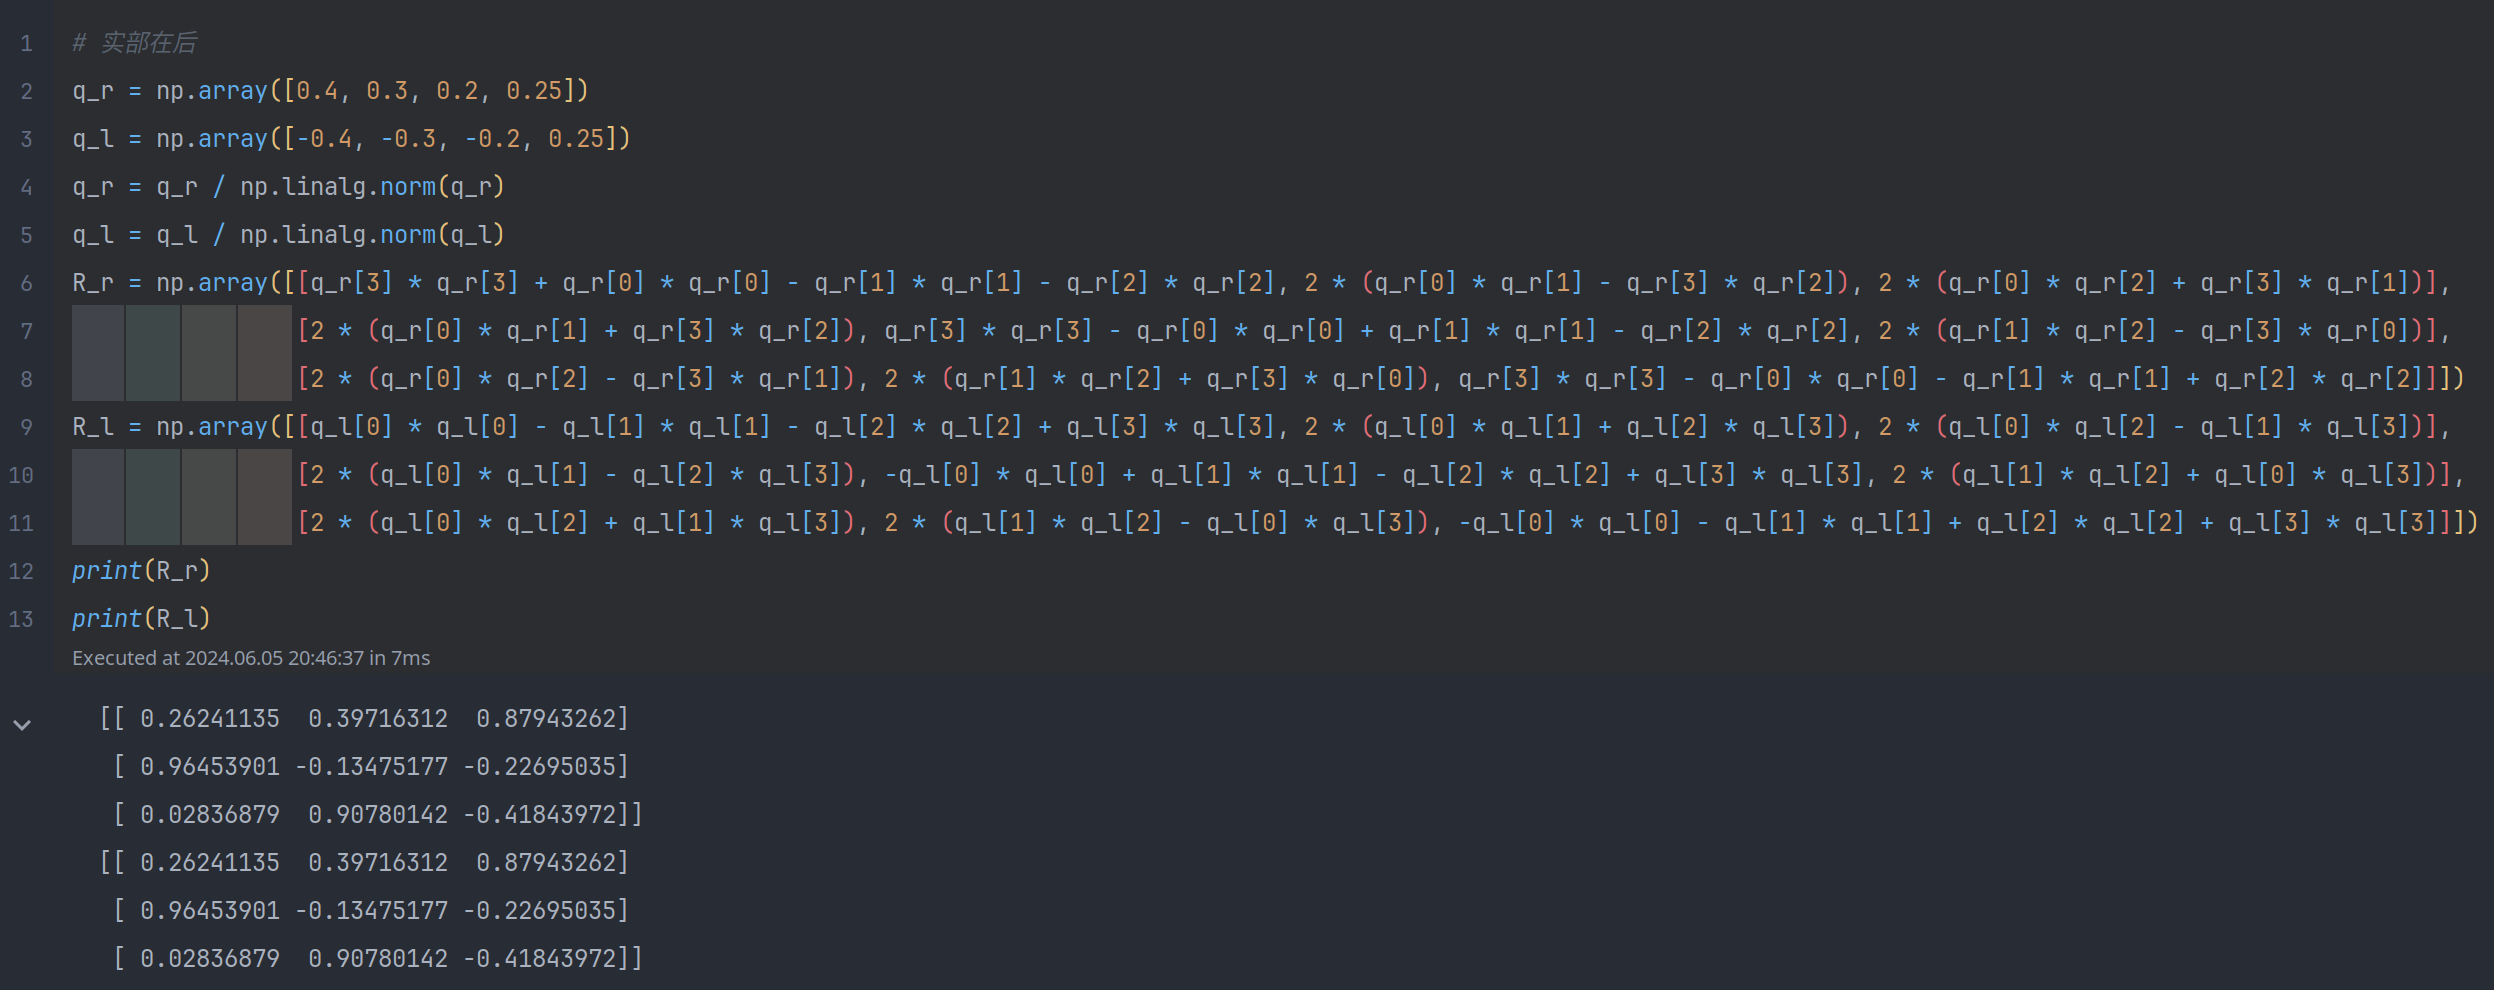
\includegraphics[width=0.85\textwidth]{figures/quaternion_comp1.png}
\captionsetup{labelformat=empty}
\caption{Figure 1.2: 满足关系$q_{left}=q^*_{right}$的四元数对应同一个旋转矩阵}
\end{figure}

\begin{figure}[ht]
\centering
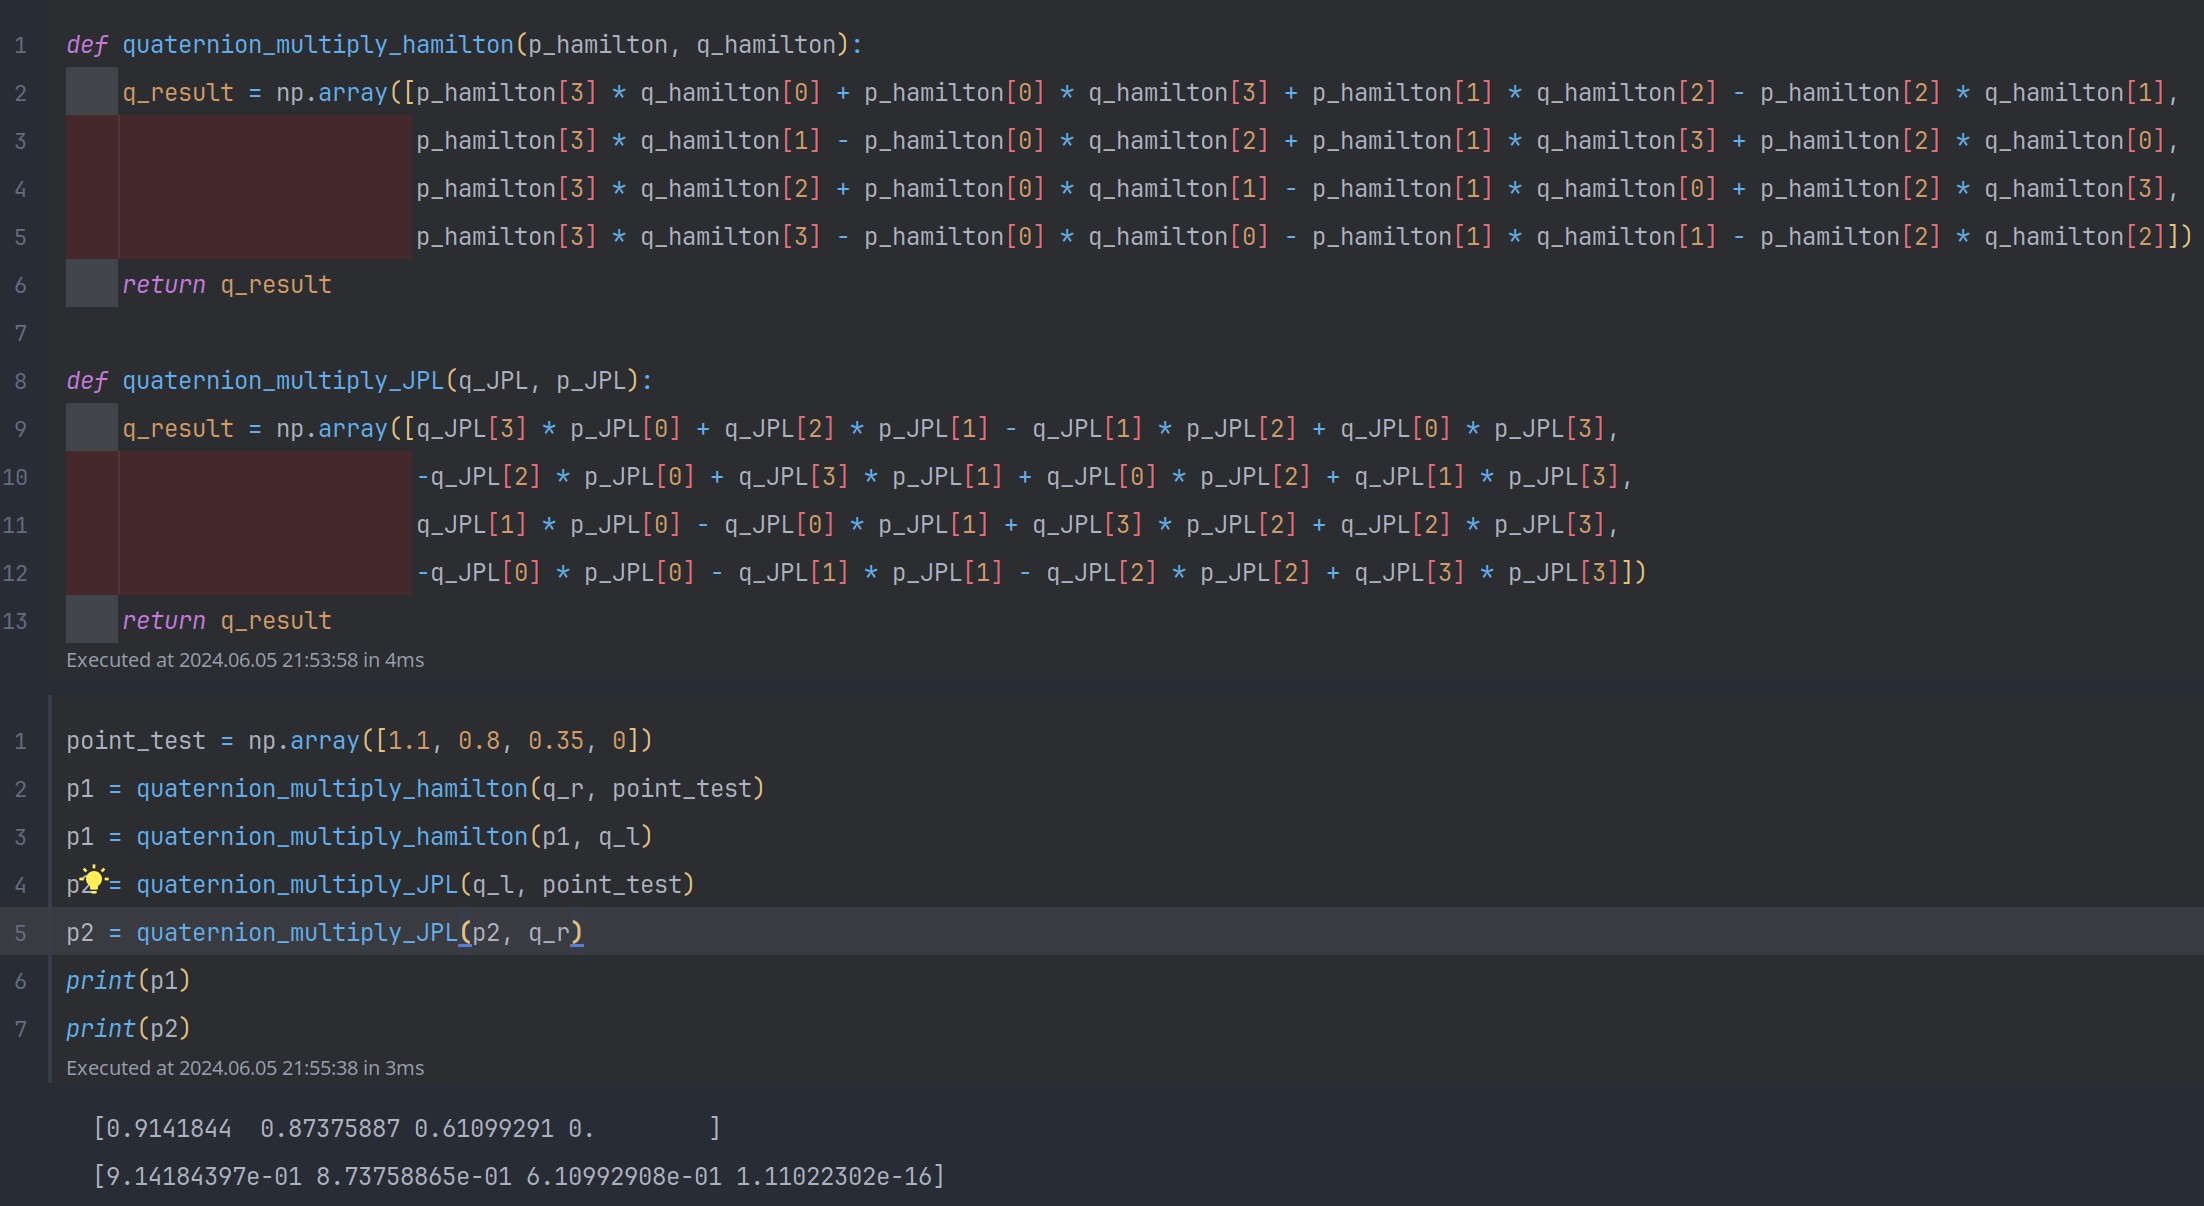
\includegraphics[width=0.85\textwidth]{figures/quaternion_comp2.png}
\captionsetup{labelformat=empty}
\caption{Figure 1.3: 满足关系$q_{left}=q^*_{right}$的四元数对点的作用是一样的}
\end{figure}

\noindent 因此,数值一样的Hamilton quaternion与JPL quaternion表示两个相反的旋转,原来Hamilton quaternion表示的旋转变换的
组合(composition),在用JPL quaternion来表示时,需要整个变换求逆。

\subsection{Propagation}

在$[t_k,t_{k+1}]$,global frame相对于

\section{第2章标题}

以下是一些样例:

\textbf{加粗文本}

\textit{倾斜文本}

\underline{下划线文本}

项目编号:

\begin{itemize}
    \item XXX
    \item XXX
    \item XXX
\end{itemize}

\begin{enumerate}
    \item XXX
    \item XXX
    \item XXX
\end{enumerate}

行内公式:$\int_a^b f(x)dx = F(b)-F(a)$

另起一行的公式:
\begin{equation}
    \int_a^b f(x)dx = F(b)-F(a)
\end{equation}

插入图片:([scale=] 中的数可以控制图片大小;后面的括号表示图片的路径,请把图片上传到figures文件夹中;caption表示图片的标题)



插入表格:
\begin{tabular}{|c|c|}% 通过添加 | 来表示是否需要绘制竖线
\hline  % 在表格最上方绘制横线
(1,1)&(1,2)\\
\hline  %在第一行和第二行之间绘制横线
(2,1)&(2,2)\\
\hline % 在表格最下方绘制横线
\end{tabular}

\subsection{小节}

在此填写小节内容

\subsubsection{小小节}

在此填写小小节内容

\

\section{结论}

在此填写结论

\

\

\section*{参考文献}

在此填写参考文献


\end{document}